\documentclass[11pt]{article}

\usepackage{"../../info/packages"}
\usepackage{"../../info/nomenclature"}
\usepackage{fullpage}


\title{ALE finite-element hydrodynamics}


\begin{document}

\maketitle

%------------------------------------------------------------------------
\section{Lagrangian governing equations}
%------------------------------------------------------------------------
We consider Lagrangian fluid particles, for which we define the position $\xvec^+=\xvec^+(t,\yvec)$, the density $\rho^+ = \rho^+(t,\yvec)$, the velocity $\uvec^+ = \uvec^+(t,\yvec)$, and the internal energy $e^+ = e^+(t,\yvec)$, where $
\yvec$ is the location of each fluid particle at time zero. The Eulerian counterparts for the density, velocity, and internal energy are, respectively, $\rho = \rho(t,\xvec)$, $\uvec = \uvec(t,\xvec)$, and $e = e(t,\xvec)$. Also consider the volume $\Omega_0$ as the set of all $\yvec$ vectors that make up the initial domain. The control volume $\Omega^+ = \Omega^+(t, \Omega_0)$ is then defined by
\begin{equation}
    \Omega^+ = \{ \xvec^+:\yvec \in \Omega_0 \}.
\end{equation}
Note that $\Omega^+(0,\Omega_0) = \Omega_0$.

The governing equations for the Lagrangian fluid particles are derived in my fluid-mechanics notes (see section on kinematics, Lagrangian governing equations, etc.). These are shown below
\begin{align}
    \frac{\partial \xvec^+}{\partial t} &= \uvec^+, \label{eq:lag_gov_evol_x} \\
    \frac{\partial J^+ \rho^+}{\partial t} &= 0, \label{eq:lag_gov_evol_rho} \\
    \rho^+ \frac{\partial \uvec^+}{\partial t} &= \left ( \nabla \cdot \sigmavec \right )_{\xvec = \xvec^+}, \label{eq:lag_gov_evol_u} \\
    \rho^+ \frac{\partial e^+}{\partial t} &= \left ( \sigmavec : \nabla \uvec \right )_{\xvec = \xvec^+}. \label{eq:lag_gov_evol_e}
\end{align}
In the above, $\sigmavec = \sigmavec(t,\xvec)$ is the stress tensor, and $J^+ = J^+(t,\yvec)$ is the determinant of the Jacobian matrix $\Jvec^+ = \Jvec^+(t,\yvec)$, which itself is defined as $\Jvec^+ =  \partial \xvec^+ / \partial \yvec$. 

A note on notation. The products that involve a tensor $\tauvec$ can be expressed in Einstein notation as
\begin{equation}
    \nabla \cdot \tauvec = \frac{\partial \tau_{ij}}{\partial x_j},
\end{equation}
\begin{equation}
    \tauvec \cdot \nabla \alpha = \tau_{ij} \frac{\partial \alpha}{\partial x_j},
\end{equation}
\begin{equation}
    \fvec \cdot \tauvec \cdot \nabla \alpha = f_i \tau_{ij} \frac{\partial \alpha}{\partial x_j},
\end{equation}
\begin{equation}
    \tauvec : \nabla \fvec = \tau_{ij} \frac{\partial f_i}{\partial x_j}.
\end{equation}
where $\alpha$ is a scalar and $\fvec$ a vector. In these notes we'll mostly be using indices $i$ and $j$ for FE expansions, rather than for Einstein notation.

%---------------------------------------------------------------
\section{Lagrangian finite elements}
%---------------------------------------------------------------
\label{sec:lag_fin_elem}
We introduce a Lagrangian basis function $\Phi_i^+ = \Phi_i^+(t,\yvec)$ and an Eulerian basis function $\Phi_i = \Phi_i(t,\xvec)$. These are related to each other as any other Lagrangian-Eulerian pair, namely 
\begin{equation}
    \label{eq:lag_fe_phi_correspondence}
    \Phi_i^+(t,\yvec) = \Phi_i(t,\xvec^+(t,\yvec)).
\end{equation}
We now introduce the Lagrangian variable $f^+ = f^+(t,\yvec)$ and the Eulerian counterpart $f = f(t,\xvec)$, and they also satisfy
\begin{equation}
    \label{eq:lag_fe_u_correspondence}
    f^+(t,\yvec) = f(t,\xvec^+(t,\yvec)).
\end{equation}
The expansion of an Eulerian variable in terms of basis functions is as follows
\begin{equation}
    \label{eq:lag_fe_expansion_eul}
    f = \sum_i^n F_i \Phi_i,
\end{equation}
where $F_i = F_i(t)$. Plugging in $\xvec^+$ for $\xvec$ in the above, and using \cref{eq:lag_fe_phi_correspondence,eq:lag_fe_u_correspondence} gives
\begin{equation}
    \label{eq:fe_lag_expansion_lag}
    f^+ = \sum_i^n F_i \Phi_i^+.
\end{equation}
Thus, both the Lagrangian and Eulerian variables share the same finite-element coefficients $F_i$. 

As shown in my fluid mechanics notes, we also have
\begin{equation}
    \label{eq:lag_fe_deriv_correspondence}
    \frac{\partial \Phi_i^+}{\partial t} = \left ( \frac{\partial \Phi_i}{\partial t} + \uvec \cdot \nabla \Phi_i \right )_{\xvec = \xvec^+},
\end{equation}
where $\uvec = \uvec(t,\xvec)$ is the Eulerian counterpart to $\uvec^+$. We'll introduce the restriction that $\Phi_i^+$ is constant in time, that is $\partial \Phi_i^+/\partial t = 0$, which gives
\begin{equation}
    \frac{\partial \Phi_i}{\partial t} + \uvec \cdot \nabla \Phi_i = 0.
\end{equation}
Thus, $F_i$ in \cref{eq:fe_lag_expansion_lag} accounts for the time dependence of $F^+$, whereas $\Phi_i^+$ accounts for the dependence on $\yvec$.

%------------------------------------------------------------------------
\section{Finite element expansion}
%------------------------------------------------------------------------
We introduce the coefficients $\hat{\xvec}_i = \hat{\xvec}_i(t)$, $\hat{\uvec}_i = \hat{\uvec}_i(t)$ and $\hat{e}_i = \hat{e}_i(t)$, as well as the Lagrangian basis functions $\phi^+_i = \phi^+_i(\yvec) \in L^2$, and $w^+_i = w^+_i(\yvec) \in H^1$. We note that $\hat{\xvec}_i$ and $\hat{\uvec}_i$ are each vectors, e.g., the components of $\hat{\uvec}_i$ are $\hat{u}_{i,\alpha} = \hat{u}_{i,\alpha}(t)$ for $\alpha = x,y,z$. We also note that $\phi^+_i$ and $w^+_i$ have Eulerian counterparts $\phi_i = \phi_i(t,\xvec)$ and $w_i = w_i(t,\xvec)$, respectively. The coefficients are used in the following expansions
\begin{equation}
    \label{eq:fe_exp_x}
    \xvec^+ = \sum_j^{N_w} \hat{\xvec}_j w^+_j,
\end{equation}
\begin{equation}
    \label{eq:fe_exp_u}
    \uvec^+ = \sum_j^{N_w} \hat{\uvec}_j w^+_j,
\end{equation}
\begin{equation}
    \label{eq:fe_exp_e}
    e^+ = \sum_j^{N_\phi} \hat{e}_j \phi^+_j.
\end{equation}
We note that the expansion coefficients are the same for the Lagrangian and Eulerian variables, as shown in \cref{sec:lag_fin_elem}. For example, for the Eulerian velocity, we have
\begin{equation}
    \uvec = \sum_j^{N_w} \hat{\uvec}_j w_j.
\end{equation}

%------------------------------------------------------------------------
\section{Semi-discrete Lagrangian governing equations}
%------------------------------------------------------------------------
%---------------------------------
\subsection{Position and Jacobian}
%---------------------------------
Plugging in \cref{eq:fe_exp_x,eq:fe_exp_u} in \cref{eq:lag_gov_evol_x} gives
\begin{equation}
    \sum_{j}^{N_w} \frac{d \hat{\xvec}_j}{dt} w^+_j = \sum_{j}^{N_w} \hat{\uvec}_j w^+_j.
\end{equation}
To satisfy the equation above, we'll require
\begin{equation}
    \frac{d \hat{\xvec}^+_j}{dt} = \hat{\uvec}_j.
\end{equation}
We now introduce the vectors $\Xvec$ and $\Uvec$, whose components are $\hat{\xvec}_i$ and $\hat{\uvec}_i$, respectively. Thus, the above is written as
\begin{equation}
    \frac{d\Xvec}{dt} = \Uvec.
\end{equation}

To obtain $\Jvec^+$ we plug in \cref{eq:fe_exp_x} into its definition, that is
\begin{equation}
    \Jvec^+ = \frac{\partial}{\partial \yvec} \sum_j^{N_w} \hat{\xvec}_j w^+_j = \sum_j^{N_w} \hat{\xvec}_j \nabla_{\yvec} w^+_j.
\end{equation}
Note that for any function $\xvec^+$, whether it be an exact analytical expression or a finite-element expansion as given by \cref{eq:fe_exp_x}, one can derive the following equation for the determinant of the Jacobian 
\begin{equation}
    \frac{\partial J^+}{\partial t} = J^+ \left ( \frac{\partial u_k}{\partial x_k} \right )_{\xvec = \xvec^+},
\end{equation}
In the above $\uvec$ is the Eulerian counterpart to $\uvec^+$, which is given by \cref{eq:lag_gov_evol_x}.

%---------------------------------
\subsection{Density}
%---------------------------------
\Cref{eq:lag_gov_evol_rho} allows us to write
\begin{equation}
    \label{eq:evol_rho_semi_discrete}
    \rho^+ = \frac{\rho^+_0}{J^+},
\end{equation}
where $\rho^+_0 = \rho^+(0,\yvec)$.

%---------------------------------
\subsection{Velocity}
%---------------------------------
Plugging in \cref{eq:evol_rho_semi_discrete} in \cref{eq:lag_gov_evol_u} we get
\begin{equation}
    \rho^+_0 \frac{\partial \uvec^+}{\partial t} = \left ( \nabla \cdot \sigmavec \right )_{\xvec = \xvec^+} J^+.
\end{equation}
We then multiply both sides of the above by the basis functions for velocity and integrate over all space to obtain
\begin{equation}
    \int_{\Omega_0} \rho^+_0 \frac{\partial \uvec^+}{\partial t} w^+_i \, dV_y = \int_{\Omega_0} \left ( \nabla \cdot \sigmavec \right )_{\xvec = \xvec^+} w^+_i J^+ \, dV_y.
\end{equation}
For the left-hand side we have
\begin{align}
    \int_{\Omega_0} \rho^+_0 \frac{\partial \uvec^+}{\partial t} w^+_i \, dV_y &= \int_{\Omega_0} \rho^+_0 \sum_j^{N_w} \frac{d \hat{\uvec}_j}{dt} w^+_j w^+_i \, dV_y, \nonumber \\
    &= \sum_j^{N_w} \frac{d \hat{\uvec}_j}{dt} \int_{\Omega_0} \rho^+_0 w^+_i w^+_j \, dV_y, \nonumber \\
    &= \sum_j^{N_w} \frac{d \hat{\uvec}_j}{dt} m_{ij}^{(w)},
\end{align}
where
\begin{equation}
    m_{ij}^{(w)} = \int_{\Omega_0} \rho^+_0 w^+_i w^+_j \, dV_y
\end{equation}
is a mass bilinear form (which is independent of time). For the right-hand side we have
\begin{align}
    \int_{\Omega_0} \left ( \nabla \cdot \sigmavec \right )_{\xvec = \xvec^+} w^+_i J^+ \, dV_y & = \int_{\Omega_0} \left ( \nabla \cdot \sigmavec w_i \right )_{\xvec = \xvec^+} J^+ \, dV_y \nonumber \\
    & = \int_{\Omega^+} \nabla \cdot \sigmavec w_i \, dV_x \nonumber \\
    & = -\int_{\Omega^+} \sigmavec \cdot \nabla w_i \, dV_x.
\end{align}
The second equality above follows from integration by substitution. Combining results we have
\begin{equation}
    \label{eq:evol_u_semi_discrete}
    \sum_j^{N_w} \frac{d \hat{\uvec}_j}{d t} m^{(w)}_{ij} = -\int_{\Omega^+} \sigmavec \cdot \nabla w_i \, dV_x.
\end{equation}

We introduce the matrix $\Mvec^{(w)}$ whose components are $m_{ij}^{(w)}$. Thus, the left-hand side of \cref{eq:evol_u_semi_discrete} can be written as $\Mvec^{(w)} \, d\Uvec / dt$.
We also introduce the vector bilinear form
\begin{equation}
    \fvec_{ij} = \int_{\Omega^+} \sigmavec \cdot \nabla w_i \phi_j \, dV_x.
\end{equation}
This is a \textit{vector} bilinear form since $\fvec_{ij}$ has components $f_{ij,\alpha} = f_{ij,\alpha}(t)$, for $\alpha = x,y,z$, where $\alpha$ denotes the first index of $\sigmavec$. We introduce the matrix $\Fvec$, whose components are $\fvec_{ij}$. We also expand the field with constant value of one as follows
\begin{equation}
    1 = \sum_i^{N_\phi} \hat{c}_i \phi_i.
\end{equation}
If we define the vector $\Cvec$ as that with components $\hat{c}_i$, we can show that 
\begin{align}
    \Fvec \Cvec &= \sum_j^{N_\phi} \fvec_{ij} \hat{c}_j \nonumber \\
    &= \sum_j^{N_\phi} \int_{\Omega^+} \sigmavec \cdot \nabla w_i \phi_j \, dV_x \hat{c}_j \nonumber \\
    &= \int_{\Omega^+} \sigmavec \cdot \nabla w_i \left ( \sum_j^{N_\phi} \hat{c}_j \phi_j \right ) \, dV_x \nonumber \\
    &= \int_{\Omega^+} \sigmavec \cdot \nabla w_i \, dV_x.
\end{align}
The above is the negative of the right-hand side of \cref{eq:evol_u_semi_discrete}. Thus, combining all together we get
\begin{equation}
    \Mvec^{(w)} \frac{d\Uvec}{dt} = -\Fvec \Cvec.
\end{equation}
We note that since both the Lagrangian and Eulerian velocities share the same coefficients $\Uvec$, we now have a solution for both.

%---------------------------------
\subsection{Energy}
%---------------------------------
Plugging in \cref{eq:evol_rho_semi_discrete} in \cref{eq:lag_gov_evol_e} we get
\begin{equation}
    \rho^+_0 \frac{\partial e^+}{\partial t} = \left ( \sigmavec : \nabla \uvec \right )_{\xvec = \xvec^+} J^+.
\end{equation}
We then multiply both sides of the above by the basis functions for energy and integrate over all space to obtain
\begin{equation}
    \int_{\Omega_0} \rho^+_0 \frac{\partial e^+}{\partial t} \phi_i^+ \, dV_y = \int_{\Omega_0} \left ( \sigmavec : \nabla \uvec \right )_{\xvec = \xvec^+} \phi_i^+ J^+ \, dV_y.
\end{equation}
For the left-hand side we have
\begin{align}
    \int_{\Omega_0} \rho^+_0 \frac{\partial e^+}{\partial t} \phi_i^+ \, dV_y &= \int_{\Omega_0} \rho^+_0 \sum_j^{N_\phi} \frac{d \hat{e}_j}{dt} \phi_j^+ \phi_i^+ \, dV_y , \nonumber \\
    &= \sum_j^{N_\phi} \frac{d \hat{e}_j}{dt} \int_{\Omega_0} \rho^+_0 \phi_j^+ \phi_i^+ \, dV_y , \nonumber \\
    &= \sum_j^{N_\phi} \frac{d \hat{e}_j}{dt} m_{ij}^{(\phi)}
\end{align}
where
\begin{equation}
    m_{ij}^{(\phi)} = \int_{\Omega_0} \rho^+_0 \phi_j^+ \phi_i^+ \, dV_y
\end{equation}
is a mass bilinear form (which is independent of time). For the right-hand side we have
\begin{align}
    \int_{\Omega_0} \left ( \sigmavec : \nabla \uvec \right )_{\xvec = \xvec^+} \phi_i^+ J^+ \, dV_y &= \int_{\Omega_0} \left ( \sigmavec : \nabla \uvec \phi_i \right )_{\xvec = \xvec^+} J^+ \, dV_y \nonumber \\
    &= \int_{\Omega^+} \sigmavec : \nabla \uvec \phi_i \, dV_x. 
\end{align}
Combining results we have
\begin{equation}
    \sum_j^{N_\phi} \frac{d \hat{e}_j}{dt} m_{ij}^{(\phi)} = \int_{\Omega^+} \sigmavec : \nabla \uvec \phi_i \, dV_x.
\end{equation}
We no show that
\begin{equation}
    \sigmavec : \nabla \uvec = \sigmavec : \nabla \left ( \sum_k^{N_w} \hat{\uvec}_k w_k \right ) = \sum_k^{N_w} \hat{\uvec}_k \cdot \sigmavec \cdot \nabla w_k,
\end{equation}
and hence the previous result is written as
\begin{equation}
    \sum_j^{N_\phi} \frac{d \hat{e}_j}{dt} m_{ij}^{(\phi)} = \sum_k^{N_w} \hat{\uvec}_k \cdot \int_{\Omega^+} \sigmavec \cdot \nabla w_k \phi_i \, dV_x.
\end{equation}
The above is finally re-written as
\begin{equation}
    \label{eq:evol_e_semi_discrete}
    \sum_j^{N_\phi} \frac{d \hat{e}_j}{d t} m^{(\phi)}_{ij} = \sum_k^{N_w} \hat{\uvec}_k \cdot \fvec_{ki}.
\end{equation}
Note that in the above there is a dot product in the right-hand side, that is, the right-hand side expanded out is  
\begin{equation}
    \sum_k^{N_w} \hat{\uvec}_k \cdot \fvec_{ki} = \sum_k^{N_w} \sum_{\alpha=x,y,z} \hat{u}_{k,\alpha} f_{ki,\alpha}.
\end{equation}

We now introduce the vector $\Evec$ whose components are $\hat{e}_i$. We also introduce the matrix $\Mvec^{(\phi)}$ whose components are $m_{ij}^{(\phi)}$. Thus, \cref{eq:evol_e_semi_discrete} can be succinctly written as
\begin{equation}
    \Mvec^{(\phi)} \frac{d\Evec}{dt} = \Fvec^T \cdot \Uvec.
\end{equation}
Note again that on the right-hand side above there is a matrix-vector product \textit{and} a dot product. We also note that since both the Lagrangian and Eulerian internal energies share the same coefficients $\Evec$, we now have a solution for both.

%------------------------------------------------------------------------
\section{Momentum and energy conservation}
%------------------------------------------------------------------------
We'll now define the internal energy $IE=IE(t)$, the kinetic energy $KE=KE(t)$, and the momentum $P_\nvec=P_\nvec(t)$ along a constant $\nvec$ direction.
\begin{align}
    IE &= \int_{\Omega^+} \rho e \, dV_x \nonumber \\
    &= \int_{\Omega_0} \rho^+ e^+ J^+ \, dV_y \nonumber \\
    &= \int_{\Omega_0} \rho^+_0 e^+ \, dV_y \nonumber \\
    &= \int_{\Omega_0} \rho_0^+ \sum_{j}^{N_\phi} \hat{e}_j \phi_j^+ \, dV_y \nonumber \\
    &= \int_{\Omega_0} \rho_0^+ \sum_{j}^{N_\phi} \hat{e}_j \phi_j^+ \left ( \sum_{i}^{N_\phi} \hat{c}_i \phi^+_i \right ) \, dV_y \nonumber \\
    &= \sum_i^{N_\phi} \sum_j^{N_\phi} \hat{c}_i \int_{\Omega_0} \rho_0^+ \phi_i^+ \phi_j^+ \, dV_y \hat{e}_j \nonumber \\
    &= \sum_i^{N_\phi} \sum_j^{N_\phi} \hat{c}_i m_{ij}^{(\phi)} \hat{e}_j \nonumber \\
    &= \Cvec \Mvec^{(\phi)} \Evec 
\end{align}

\begin{align}
    KE &= \int_{\Omega^+} \frac{1}{2} \rho \uvec \cdot \uvec \, dV_x \nonumber \\
    &= \int_{\Omega_0} \frac{1}{2} \rho^+ \uvec^+ \cdot \uvec^+ J^+ \, dV_y \nonumber \\
    &= \int_{\Omega_0} \frac{1}{2} \rho_0^+ \uvec^+ \cdot \uvec^+ \, dV_y \nonumber \\
    &= \int_{\Omega_0} \frac{1}{2} \rho_0^+ \left ( \sum_i^{N_w} \hat{\uvec}_i w_i^+ \right ) \cdot \left ( \sum_j^{N_w} \hat{\uvec}_j w_j^+ \right ) \, dV_y \nonumber \\
    &= \sum_i^{N_w} \sum_j^{N_w} \frac{1}{2} \hat{\uvec}_i \cdot \int_{\Omega_0}\rho_0^+ w_i^+ w_j^+ \, dV_y \hat{\uvec}_j \nonumber \\
    &= \sum_i^{N_w} \sum_j^{N_w} \frac{1}{2} \hat{\uvec}_i \cdot m_{ij}^{(w)} \hat{\uvec}_j \nonumber \\
    &= \frac{1}{2} \Uvec \cdot \Mvec^{(w)} \Uvec.
\end{align}

\begin{align}
    P_\nvec &= \int_{\Omega^+} \rho \uvec \cdot \nvec \, dV_x \nonumber \\
    &= \int_{\Omega_0} \rho^+ \uvec^+ \cdot \nvec J^+ \, dV_y \nonumber \\
    &= \int_{\Omega_0} \rho^+_0 \uvec^+ \cdot \nvec \, dV_y \nonumber \\
    &= \int_{\Omega_0} \rho^+_0 \left ( \sum_j^{N_w} \hat{\uvec}_j w^+_j \right ) \cdot \left ( \sum_i^{N_w} \hat{\nvec}_i w_i^+ \right ) \, dV_y \nonumber \\
    &= \sum_i^{N_w} \sum_j^{N_w} \hat{\nvec}_i \cdot \int_{\Omega_0} \rho_0^+ w_i^+ w_j^+ \, dV_y \hat{\uvec}_j \nonumber \\
    &= \sum_i^{N_w} \sum_j^{N_w} \hat{\nvec}_i \cdot m_{ij}^{(w)} \hat{\uvec}_j \nonumber \\
    &= \Nvec \cdot \Mvec^{(w)} \Uvec.
\end{align}

The total energy is conserved, as shown below
\begin{align}
    \frac{d}{dt} (IE + KE) &= \Cvec \Mvec^{(\phi)} \frac{d\Evec}{dt} + \Uvec \cdot \Mvec^{(w)} \frac{d\Uvec}{dt} \nonumber \\
    &= \Cvec \Fvec^T \cdot \Uvec - \Uvec \cdot \Fvec \Cvec \nonumber \\
    &= 0.
\end{align}
The momentum along a constant direction is conserved, as shown below
\begin{align}
    \frac{d P_\nvec}{dt} &= \Nvec \cdot \Mvec^{(w)} \frac{d \Uvec}{dt} \nonumber \\
    &= -\Nvec \cdot \Fvec \Cvec \nonumber \\
    &= -\sum_i^{N_w} \sum_j^{N_\phi} \hat{\nvec}_i \cdot \fvec_{ij} \hat{c}_j \nonumber \\
    &= -\sum_i^{N_w} \sum_j^{N_\phi} \hat{\nvec}_i \cdot \int_{\Omega^+} \sigmavec \cdot \nabla w_i \phi_j \, dV_x \hat{c}_j \nonumber \\
    &= -\int_{\Omega^+} \sigmavec : \nabla \nvec \, dV_x \nonumber \\
    &= 0.
\end{align}

%------------------------------------------------------------------------
\section{The reference element}
%------------------------------------------------------------------------
\begin{table}
    \centering
    \begin{tabular}{c|c}
          full domain & element's domain \\
          \hhline{=|=}
          $\Omega_0$ & $\Omega_{0,e}$ \\
          $\Omega^+$ & $\Omega^+_e$ \\
          $\xvec^+$ & $\xvec^+_e$ \\
          $J^+$ & $J^+_e$
    \end{tabular}
    \caption{Mapping within an element}
    \label{tab:map_element}
\end{table}
We consider a subset of $\Omega_0$, namely $\Omega_{0,e}$, which consists of a single element in the mesh at time zero. At some later time, the domain of this single element could have changed, and it is then given by $\Omega^+_e = \Omega^+_e(t,\Omega_{0,e})$. Whereas $\xvec^+$ maps from $\Omega_0$ to $\Omega^+$, the variable $\xvec^+_e$ maps from $\Omega_{0,e}$ to $\Omega^+_e$. The corresponding determinant of the Jacobian is $J^+_e$. A summary of these new variables is given in \cref{tab:map_element}.

\begin{figure}[ht]
    \centering
    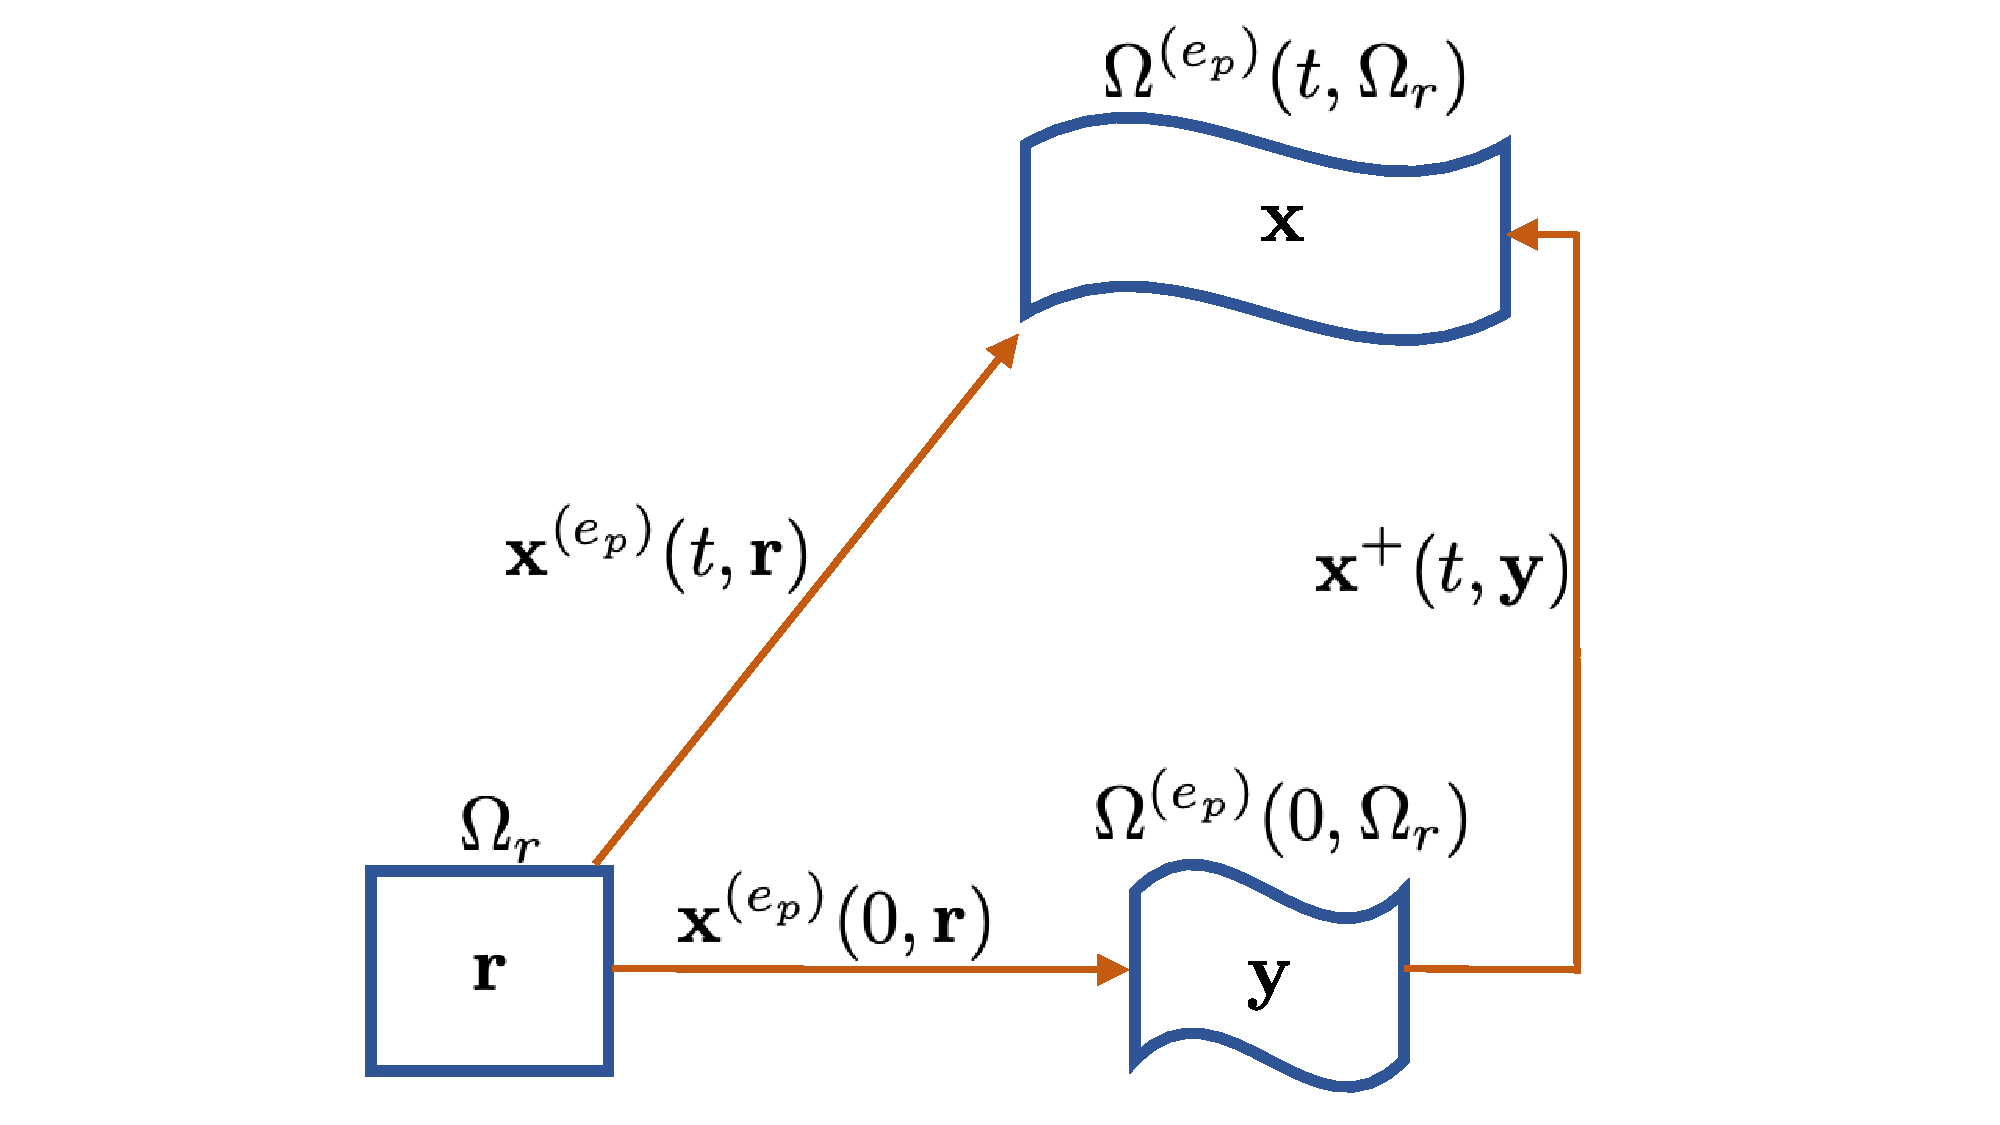
\includegraphics[width=0.7\textwidth]{../../images/three_spaces.pdf}
    \caption{Schematic of the three domains $\Omega_{0,e}$, $\Omega^+_e$, $\Omega_z$.}
    \label{fig:three_spaces}
 \end{figure}
We also introduce the reference element as the unit square in 2D or the unit sphere in 3D. This element is labelled as $\Omega_z$ and it doesn't change with time. We introduce the mapping function $\Phivec_e = \Phivec_e(t,\zvec)$, which maps from points $\zvec$ in $\Omega_z$ to points in $\Omega^+_e$. A depiction of these domains and their mappings is shown in \cref{fig:three_spaces}. A condition satisfied by $\Phivec_e$ is
\begin{equation}
    \Phivec_e(t,\zvec) = \xvec^+_e(t, \Phivec_e(0,\zvec)).
\end{equation}
We can also define the Jacobian $\Jvec_z = \Jvec_z(t,\zvec)$ as $\Jvec_z = \partial \Phivec_e / \partial \zvec$, and label its determinant as $J_z = J_z(t,\zvec)$. Thus, the volume of a single element can now be computed using either of the three integrals below
\begin{equation}
    \text{vol}_e = \int_{\Omega^+_e} dV_x = \int_{\Omega_{0,e}} J^+_e \, dV_y = \int_{\Omega_z} J_z \, dV_z.
\end{equation}

\end{document}